
\part*{{\huge Differentialrechnung}}


\section*{{\large Grenzwert und Stetigkeit}}


\subsection*{Symmetrien:}
\begin{quote}
\begin{tabular}{|l||l|}
\hline 
y-Achsensymmetrie: f(x)=f(-x) & Punktsymmetrie: f(x)=-f(-x)\tabularnewline
\hline 
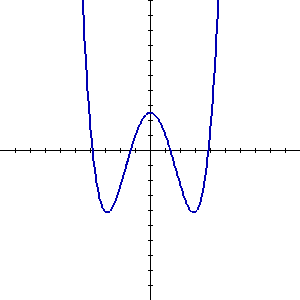
\includegraphics[width=4cm]{Differentialrechnung/achsensymm1} & 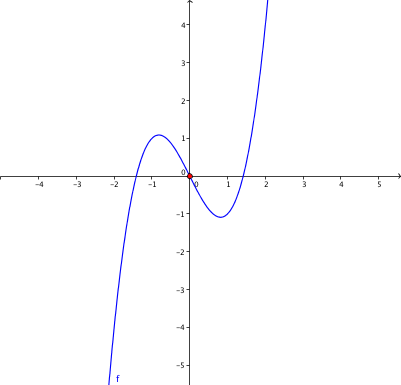
\includegraphics[width=4cm]{Differentialrechnung/Punktsym.jpg}\tabularnewline
\hline 
\end{tabular}
\end{quote}

\subsection*{Grenzwert bei Definitionslücken}
\begin{quote}
\begin{tabular}{|c|c|}
\hline 
Bsp: $f:y=\frac{x^{2}-1}{x-1}$, $D=R\setminus\left\{ 1\right\} $ & Bsp: $f:y=\frac{sin(x)}{x}$, $D=R\setminus\left\{ 0\right\} $\tabularnewline
\hline 
Kürzen möglich: $f:y=x+1$, & Kürzen nicht möglich\tabularnewline
\hline 
Definitionslücke: $x=1$ & Definitionslücke: $x=0$\tabularnewline
\hline 
Art: hebbar & Art: normale (nicht hebbare)\tabularnewline
\hline 
$lim_{x\rightarrow1}(x+1)=2$ & $lim_{x\rightarrow0}(\frac{sin(x)}{x})=1$\tabularnewline
\hline 
\end{tabular}
\end{quote}

\subsection*{Konvergenz}
\begin{quote}
Als $lim_{x\rightarrow x_{0}}f(x)=g$ - Aussage: $f(x)$ konvergiert
für $x$ gegen $x_{0}$ gegen den Grenzwert $g$ ($\ni R$).

$\forall\varepsilon\exists\delta:\forall x\mid x-x_{0}\mid<\delta,\mid f(x)-g\mid<\varepsilon$,
$g$ Grenzwert, dann konvergiert die Funktion gegen $g$
\end{quote}

\subsection*{Divergenz}
\begin{itemize}
\item Polstelle ($lim_{x\rightarrow x_{0}}=_{-}^{+}\infty$)
\item Sprung ($lim_{-\rightarrow x_{0}}\neq lim_{+\rightarrow x_{0}}$)
\item oszilliert
\end{itemize}

\subsection*{Stetigkeit}
\begin{quote}
Definition: $lim_{x\rightarrow x_{0}}f(x)=f(x_{0})$, dann ist die
Funktion stetig in $x_{0}$.\end{quote}
\begin{itemize}
\item Alle Polynome in $R$ sind stetig
\item Alle gebrochen-rationalen Funktionen in $R$ sind stetig (ausser Nullstellen
des Nenners)
\item Ist $f(x)$ in einem Intervall stetig, so ist auch $f(x)^{n}$ und
$e^{f(x)}$ im selben Intervall stetig
\end{itemize}

\section*{Grundlagen der Diff.rechnung}


\subsection*{Differenzenquotient}
\begin{verse}
\begin{tabular}{|c|}
\hline 
$Geradensteigung=m=tan(\alpha)=\frac{\Delta f}{\Delta x}=\frac{f(x_{0}+\Delta x)-f(x_{0})}{\Delta x}=\frac{y-\ddot{A}nderung}{x-\ddot{A}nderung}=\frac{y_{1}-y_{0}}{x_{1}-x_{0}}$\tabularnewline
\hline 
\end{tabular}
\end{verse}

\subsection*{Differentialquotient}
\begin{verse}
\begin{tabular}{|c|}
\hline 
$Differentialquotien=lim(Differenzenquotient)=lim_{\Delta x\rightarrow0}\frac{\Delta f(x)}{\Delta x}=lim_{\Delta x\rightarrow0}\frac{f(x_{0}+\Delta x)-f(x_{0})}{\Delta x}$\tabularnewline
\hline 
\end{tabular}
\end{verse}
Existiert de Differentialquotient so heisst die Funktion $f(x)$ an
der Stelle $x_{0}$ differenzierbar. Geometrisch bedeutet die Ableitund
der Funktion an einer Stelle deren Tangentensteigung.


\subsection*{Ableitungsfunktion}

Beispiel: Finden der abgeleiteten Funktion mit Diff.quot.:

\[
f(x)=x^{2},Diff.quot=m=\frac{f(x_{0}+\Delta x)-f(x_{0})}{\Delta x}
\]


\[
Diff.quot=\frac{(x_{0}+\Delta x)^{2}-(x_{0})^{2}}{\Delta x}=\frac{2x_{0}\Delta x+\Delta x^{2}}{\Delta x}=2x_{0}+\Delta x
\]


\[
f'(x)=lim_{\Delta x\rightarrow0}(2x_{0}+\Delta x)=2x_{0}
\]


Orte, an denen dieser Grenzwert nicht existieren kann:
\begin{itemize}
\item Graph hat eine Ecke oder Knick: $lim(links)\neq lim(rechts)$ deshalb
hat $f'(x)$ einen Sprung bei $x_{0}$.
\item Der Graph kann eine senkrechte Tangente aufweisen: $lim(f(x))=\infty$.
\end{itemize}

\subsubsection*{Tangente}
\begin{quote}
$Tangente(f(x))=f'(x)$
\end{quote}

\subsubsection*{Normale}
\begin{quote}
$Normale(f(x))=\frac{-1}{f'(x)}$
\end{quote}

\subsection*{Linearisierung}

Eine NICHT lineare Funktion $y=f(x)$ lässt sich in der Umgebung eines
Kurvenpunktes $P(x_{0},y_{0})$ durch die dortige Tangente ersetzen.

\[
\frac{y-y_{0}}{x-x_{0}}=f'(x)\Rightarrow y-y_{0}=f'(x_{0})(x-x_{0})\Rightarrow y=y_{0}+f'(x_{0})(x-x_{0})
\]


\[
f(x_{0}+\Delta x)\simeq y_{0}+f'(x_{0})\times\Delta x)
\]


Bsp:

\begin{tabular}{|c|c|c|cc}
\cline{1-1} \cline{3-3} 
$f(x)=x^{3}$ &  & $f'(x)=3x^{2}$ &  & \tabularnewline
\cline{1-1} \cline{3-3} 
$x_{0}=1$ & \multicolumn{1}{c}{} & \multicolumn{1}{c}{} &  & $f(1.01)\approx f(1)+f'(1)\times0.01=1.03$\tabularnewline
\cline{1-1} \cline{3-3} 
$f(1)=y_{0}=1$ &  & $f'(1)=3$ &  & $f(1.01)=(1.01)^{3}=1.030301$\tabularnewline
\cline{1-1} \cline{3-3} 
\multicolumn{1}{c}{} & \multicolumn{1}{c}{} & \multicolumn{1}{c}{} &  & Fehler: $0.3\permil$\tabularnewline
\end{tabular}


\subsection*{Ableitungsregeln}
\begin{quote}
\begin{tabular}{|c|c|c|c|c|c|c|}
\cline{1-3} \cline{5-7} 
$(c)'=c$ & $ln(x)'=\frac{1}{x}$ & $sin'=cos$ &  & $f(x)=c\cdot g(x)$ & $\implies$ & $f'(x)=c\cdot g'(x)$\tabularnewline
\cline{1-3} \cline{5-7} 
$(x^{n})'=n\cdot x^{n-1}$ & $(e^{x})'=e^{x}$ & $cos'=-sin$ &  & $f(x)=u(x)+v(x)$ & $\implies$ & $f'(x)=u'(x)+v'(x)$\tabularnewline
\cline{1-3} \cline{5-7} 
 & $(a^{x})'=a^{x}\cdot ln(a)$ & $tan'=\frac{1}{cos^{2}}$ &  & $f(x)=u(x)\cdot v(x)$ & $\implies$ & $f'(x)=u'\cdot v+u\cdot v'$\tabularnewline
\cline{2-3} \cline{5-7} 
 & $(log_{a}x)'=\frac{1}{x\cdot ln(a)}$ & $arctan'=\frac{1}{1+x^{2}}$ &  & $f(x)=\frac{u(x)}{v(x)}$ & $\implies$ & $f'(x)=\frac{u'\cdot v-u\cdot v'}{v^{2}}$\tabularnewline
\cline{3-3} \cline{5-7} 
 &  & $arcsin'=\frac{1}{\sqrt{1-x^{2}}}$ &  & $f(x)=g(h(x))$ & $\implies$ & $f'(x)=g'(h)\cdot h'(x)$\tabularnewline
\cline{3-3} \cline{5-7} 
 &  & $arccos'=\frac{-1}{\sqrt{1-x^{2}}}$ &  & $(f^{-1})'$ & $=$ & $\frac{1}{f'(x_{0})}$\tabularnewline
\end{tabular}
\end{quote}

\section*{Untersuchung von Funktionen}


\subsection*{Aussagen der 1ten Ableitung}
\begin{quote}
$f(x)$ in Intervall $I$ differenzierbar, dann:\end{quote}
\begin{itemize}
\item $f'(x)=0$ : Extremum (min/max) auf dem Intervall $I$
\item $f'(x)>0$ : $f(x)$ in $I$ monoton wachsend
\item $f'(x)<0$ : $f(x)$ in $I$ monoton fallend\end{itemize}
\begin{quote}
Das heisst, dass das Vorzeichen der ersten Ableitung uns sagt, ob
die Funktion steigt oder fällt.
\end{quote}

\subsection*{Aussagen der 2ten Ableitung}
\begin{quote}
$f(x)$ in Intervall $I$ 2 mal differenzierbar, dann:\end{quote}
\begin{itemize}
\item \textbf{$f''(x)>0$} : $f'(x)$ ist (streng) monoton wachsend : $f(x)$
ist \textbf{konvex}
\item \textbf{$f''(x)<0$ }: $f'(x)$ ist (streng) monoton fallend : $f(x)$
ist \textbf{konkav}
\end{itemize}

\subsection*{Extremwerte}
\begin{quote}
Durch die erste Ableitung $f'(x)=0$ erhalten wir Kandidatstellen
$x_{i}$ für Minimum und Maximum.\end{quote}
\begin{itemize}
\item Ist in der Umgebung der Stelle $x_{i}$ die Funktion $f(x)$ \textbf{konkav},
so liegt ein \textbf{Maximum} vor.
\item Ist in der Umgebung der Stelle $x_{i}$ die Funktion $f(x)$ \textbf{konvex},
so liegt ein \textbf{Minimum} vor.
\end{itemize}

\subsection*{Wendepunkte}
\begin{quote}
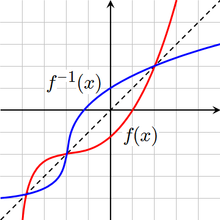
\includegraphics[width=4cm]{Differentialrechnung/220px-Inverse_Function_Graph}$f(x)$
ist im Intervall $I$ 3 mal differenzierbar, dann:\end{quote}
\begin{itemize}
\item $f''=0,f'''<0$ : blau : Links- zu Rechtskurve
\item $f''=0,f'''>0$ : rot : Rechts- zu Linkskurve
\end{itemize}

\section*{Newtonverfahren}
\begin{quote}
Newtonsches Tangentenverfahren:
\[
x_{n}=x_{n-1}-\frac{f(x_{n-1})}{f'(x_{n-1})},n=1,2,3,...
\]


Kriterium, das für Startwert und während des ganzen Verfahrens gelten
soll:
\[
\mid\frac{f\cdot\text{f'}}{(f'')^{2}}\mid<1
\]


Startwert: nicht Stellen, an denen die Kurventangente (fast) parallel
zur x-Achse verläuft.
\end{quote}

\section*{Bernoulli de l'Hopital}


\subsection*{Mittelwertsatz der Diff.rechnung}

\begin{tabular}{|c|c|}
\hline 
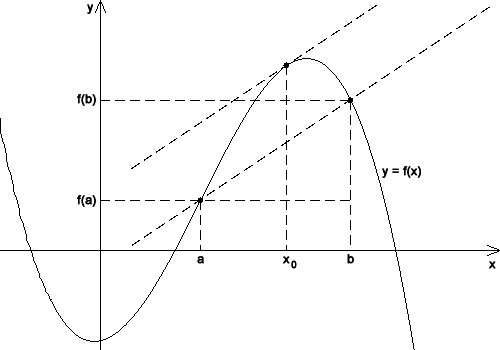
\includegraphics[width=5cm]{Differentialrechnung/MittelwertsatzD} & \includegraphics[width=5cm]{Differentialrechnung/550px-Satz_von_Rolle\lyxdot svg}\tabularnewline
\hline 
\hline 
$f(x)$ in $[a,b]$ stetig und differenzierbar in $]a,b[$ , dann
$\exists\xi\in]a,b[$ : & Spezialfall: Satz von Rolle \tabularnewline
\hline 
$\frac{f(b)-f(a)}{b-a}=f'(\xi)$ & $f(a)=f(b)$\tabularnewline
\hline 
\end{tabular}


\subsection*{Allgemeiner Mittelwertsatz der Diff.rechnung}
\begin{quote}
$f(x),g(x)$ in $[a,b]$ stetig und in$]a,b[$ differenzierbar sowie
$g'(x)\neq0$ in $]a,b[$, dann $\exists\xi\in]a,b[$:

\[
\frac{f(b)-f(a)}{g(b)-g(a)}=\frac{f'(\xi)}{g'(\xi)}
\]

\end{quote}

\subsection*{Regel von Bernoulli de l'Hopital}
\begin{quote}
Die Funktionen seien auf einen offenen Intervall stetig: $]a,b[$
(wobei das Intervall auch unendlich sein kann).

Falls:
\[
lim_{x\rightarrow b}f(x)=lim_{x\rightarrow b}g(x)=0\: oder\: lim_{x\rightarrow b}f(x)=lim_{x\rightarrow b}g(x)=_{-}^{+}\infty\: und\: lim_{x\rightarrow b}\frac{f'}{g'}=d
\]


so ist: 
\[
lim_{x\rightarrow b}\frac{f(x)}{g(x)}=lim_{x\rightarrow b}\frac{f'(x)}{g'(x)}=d
\]
\end{quote}

